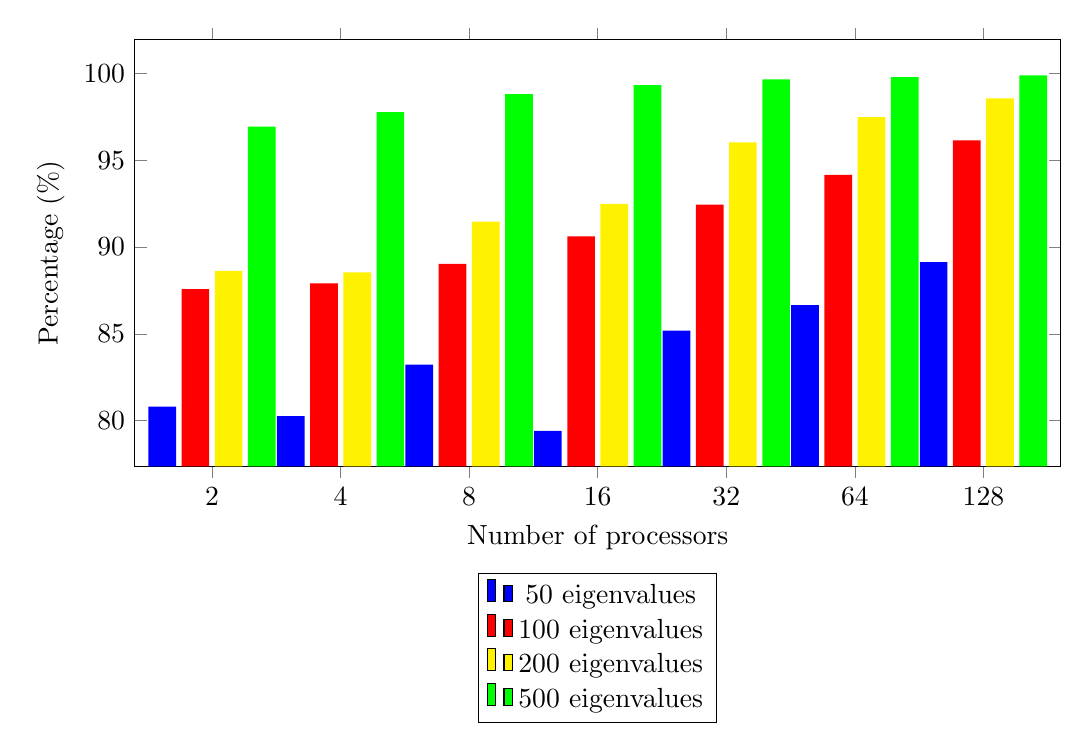
\begin{tikzpicture}
 \begin{axis}[
  ybar,
  height=7cm,
  width=1.1\textwidth,
  xlabel=Number of processors,
  xtick={0, 1, 2, 3, 4, 5, 6},
  xticklabels={2, 4, 8, 16, 32, 64, 128},
  legend style={
   at={(0.5, -0.25)},
   anchor=north
  },
  ylabel={Percentage (\%)}]
  \addplot[draw=none, fill=blue] coordinates {
   (0, 80.81)
   (1, 80.26)
   (2, 83.23)
   (3, 79.41)
   (4, 85.19)
   (5, 86.65)
   (6, 89.13)};
  \addplot[draw=none, fill=red] coordinates {
   (0, 87.57)
   (1, 87.90)
   (2, 89.03)
   (3, 90.61)
   (4, 92.44)
   (5, 94.15)
   (6, 96.14)};
  \addplot[draw=none, fill=yellow] coordinates {
   (0, 88.62)
   (1, 88.54)
   (2, 91.46)
   (3, 92.49)
   (4, 96.02)
   (5, 97.48)
   (6, 98.56)};
  \addplot[draw=none, fill=green] coordinates {
   (0, 96.93)
   (1, 97.77)
   (2, 98.81)
   (3, 99.32)
   (4, 99.65)
   (5, 99.79)
   (6, 99.89)};
  \legend{
   50 eigenvalues,
   100 eigenvalues,
   200 eigenvalues,
   500 eigenvalues}
 \end{axis}
\end{tikzpicture}
